% Template for ICASSP-2019 paper; to be used with:
%          spconf.sty  - ICASSP/ICIP LaTeX style file, and
%          IEEEbib.bst - IEEE bibliography style file.
% --------------------------------------------------------------------------
\documentclass{article}
\usepackage{spconf,amsmath,graphicx,epstopdf,float}

% Example definitions.
% --------------------
\def\x{{\mathbf x}}
\def\L{{\cal L}}

\title{Multi-scale Defect Detection Network for Tire X-ray Images}


\name{Ren Wang{\rm\textsuperscript{1,2}}, Qiang Guo{\rm\textsuperscript{1,2}}, Shanmei Lu{\rm\textsuperscript{1,2}}, Caiming Zhang{\rm\textsuperscript{3}}}

\address{\textsuperscript{1}School of Computer Science and Technology, \\Shandong University of Finance and Economics, Jinan, China\\
        \textsuperscript{2}Shandong Provincial Key Laboratory of Digital Media Technology, Jinan, China\\
        \textsuperscript{3}Software College, Shandong University, Jinan, China}


\begin{document}
%\ninept

\maketitle

\begin{abstract}
Though automatic detection method has been tremendous improved, with the gradual penetration of deep learning. Defect detection in many industrial processes is one of the remaining challenging tasks due to the diversity of its products. In this work, we focus on detection tasks in tire industry and develop a {\it Multi-scale Defect Detection Network (MDDN)}, which contains two parallel sub-networks to capture multi-scale defect features. Specifically, high-abstracted semantic features containing defect shapes and locations are mined via a {\it Semantic-aware sub-network}, simplified by an off-the-shelf fully convolutional network. Furthermore, to complement the details filtered by the deep network, a novel {\it Texture-aware Sub-network} is used to exploit the small size of the cover edge features and small defects as much as possible. Finally, the pixel-wised detection results are obtained by fusing features with semantic and texture information. Extensive experiments demonstrate that {\it MDDN} can produce comparable results and achieve significantly performance improvement in small defects detection.
\end{abstract}

\begin{keywords}
Defect detection, Fully convolutional network, Semantic segmentation, Multi-scale context
\end{keywords}

\section{Introduction}
\label{sec:intro}
Automatic defect detection, used to improve quality and accelerate production, has become an indispensable part in industrial processes, such as fabrics\cite{kumar2008computer,ngan2011automated,li2016deformable}, steel\cite{ghorai2012automatic}, semiconductors\cite{bai2014saliency}, and solar wafers\cite{tsai2012defect}. Especially in tire manufacturing, numerous detection algorithms have been proposed\cite{zhang2013texture,cui2016defect,cui2016novel,zhang2018tire,guo2016defect} and aroused extensive attention over the past two decades. In most real-world applications, tire defect detection is first carried out by deriving the defective region from tire X-ray images, which contains various types of defects caused by unclean raw materials and undesired manufacturing facilities\cite{guo2012tire}. Then, the defective product is hierarchical processed according to the location and size of defects. Due to unique properties of the tire image, for instance complexity and low-quality, illustrated in previous study\cite{zhang2013defect,wang2019tire}, most inspection processes are performed by human observers, which increases the risk and reduces the efficiency. Therefore, tire defect detection remains one of the most challenging inspection tasks.

\begin{figure}[t]
  \centering
  \centerline{\includegraphics[width=9cm]{pic1.eps}}
  \caption{Detection results of several benchmark architecture. (a) shows input tire images with different defects. From top to bottom, the first four are tire sidewall images, which involve following defect types: impurity, overlap, slack, bubble. The last two are tire tread images, which involve overlaps. }
\end{figure}

At present, existing computer vision based detection methods are mostly devoted to distinguish difference between defective regions and background (defective-free regions). Hence a key issue for such methods is feature extraction. Guo {\it et al}.\cite{guo2016defect} exploited a local kernel regression descriptor to derive feature vectors. By comparing the dissimilarity of the corresponding feature between one pixel and its neighbors, anomaly pixels can be located and segmented, even in the tread image. Nevertheless, this method is not suitable for real-time detection tasks because of the high computational complexity. A component decomposition based method was proposed in\cite{guo2012tire}, which separated the background from the image by means of two designed filters. Then through an adaptive thresholding processing, defects were derived from the residual image. Besides, Independent component analysis(ICA) was also used for defect detection tasks\cite{cui2016defect,cui2016novel}. A major disadvantage of these fundamental methods is the limitation of the information contained in low-level clues and domain features. To address the limitation, Zhang {\it et al}.\cite{zhang2013texture} and Zhang {\it et al}.\cite{zhang2013defect} introduced radon transform and mulit-scale transform, for instance curvelet and wavelet transform, in detection tasks respectively. Furthermore, optimized edge detection and total variation algorithm are used to achieve more accurate results\cite{yan2013detection}. Zhao {\it et al}.\cite{zhao2017tire} proposed a multiple kernel learning method, which combined various transform kernels to get more differentiated information. However, the representation capability of fixed kernels is not comprehensive enough. In addition, transform process is computationally expensive. Recently, Cui {\it et al}.\cite{cui2018tire} attempted to classify tire defects by means of convolutional neural networks(CNN), which has outstanding performance in the recognition and segmentation tasks of natural images. With the excellent feature extraction capability of deep network, Wang {\it et al}.\cite{wang2019tire} further implemented the detection and segmentation in tire images by a fully convolutional network(FCN)\cite{long2015fully}. However, FCN is not sensitive to small defects and edge details, which is similar to that in dealing with natural image tasks.



%\Figure[t!][width=0.86\textwidth]{test1.eps}
%{Detection results of several benchmark architecture. (a) shows input tire images with different defects. From top to bottom, the first four are tire sidewall images, which involve following defect types: impurity, overlap, slack, bubble. The last two are tire tread images, which involve overlaps. (b) indicates ground truths obtained by manual marking. (c),(d),(e) and (f) are detection results using AlexNet, VGG11, VGG13 and VGG16 as the basic architecture, respectively. \label{fig1}}

\section{Multi-scale Defect Detection Network}
\label{sec:format}

All printed material, including text, illustrations, and charts, must be kept
within a print area of 7 inches (178 mm) wide by 9 inches (229 mm) high. Do
not write or print anything outside the print area. The top margin must be 1
inch (25 mm), except for the title page, and the left margin must be 0.75 inch
(19 mm).  All {\it text} must be in a two-column format. Columns are to be 3.39
inches (86 mm) wide, with a 0.24 inch (6 mm) space between them. Text must be
fully justified.

\section{EXPERIMENTS}
\label{sec:pagestyle}

The paper title (on the first page) should begin 1.38 inches (35 mm) from the
top edge of the page, centered, completely capitalized, and in Times 14-point,
boldface type.  The authors' name(s) and affiliation(s) appear below the title
in capital and lower case letters.  Papers with multiple authors and
affiliations may require two or more lines for this information. Please note
that papers should not be submitted blind; include the authors' names on the
PDF.

\section{CONCLUSION}
\label{sec:typestyle}

To achieve the best rendering both in printed proceedings and electronic proceedings, we
strongly encourage you to use Times-Roman font.  In addition, this will give
the proceedings a more uniform look.  Use a font that is no smaller than nine
point type throughout the paper, including figure captions.

In nine point type font, capital letters are 2 mm high.  {\bf If you use the
smallest point size, there should be no more than 3.2 lines/cm (8 lines/inch)
vertically.}  This is a minimum spacing; 2.75 lines/cm (7 lines/inch) will make
the paper much more readable.  Larger type sizes require correspondingly larger
vertical spacing.  Please do not double-space your paper.  TrueType or
Postscript Type 1 fonts are preferred.

The first paragraph in each section should not be indented, but all the
following paragraphs within the section should be indented as these paragraphs
demonstrate.


\subsubsection{Sub-subheadings}
\label{sssec:subsubhead}

In LaTeX, to start a new column (but not a new page) and help balance the
last-page column lengths, you can use the command ``$\backslash$pagebreak'' as
demonstrated on this page (see the LaTeX source below).



Since there are many ways, often incompatible, of including images (e.g., with
experimental results) in a LaTeX document, below is an example of how to do
this \cite{Lamp86}.

List and number all bibliographical references at the end of the
paper. The references can be numbered in alphabetic order or in
order of appearance in the document. When referring to them in
the text, type the corresponding reference number in square
brackets as shown at the end of this sentence \cite{C2,kumar2008computer}. An
additional final page (the fifth page, in most cases) is
allowed, but must contain only references to the prior
literature.

These guidelines include complete descriptions of the fonts, spacing, and
related information for producing your proceedings manuscripts. Please follow
them and if you have any questions, direct them to Conference Management
Services, Inc.: Phone +1-979-846-6800 or email
to \\\texttt{icassp2019@cmsworkshops.com}.

% Below is an example of how to insert images. Delete the ``\vspace'' line,
% uncomment the preceding line ``\centerline...'' and replace ``imageX.ps''
% with a suitable PostScript file name.
% -------------------------------------------------------------------------
\begin{figure}[htb]

\begin{minipage}[b]{1.0\linewidth}
  \centering
  \centerline{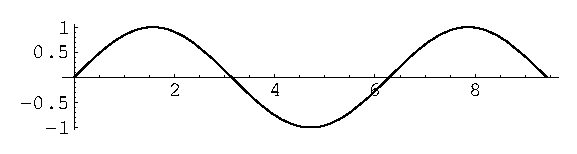
\includegraphics[width=8.5cm]{image1.eps}}
%  \vspace{2.0cm}
  \centerline{(a) Result 1}\medskip
\end{minipage}
%
\begin{minipage}[b]{.48\linewidth}
  \centering
  \centerline{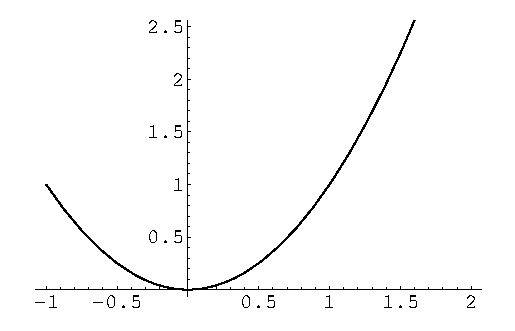
\includegraphics[width=4.0cm]{image3.eps}}
%  \vspace{1.5cm}
  \centerline{(b) Results 3}\medskip
\end{minipage}
\hfill
\begin{minipage}[b]{0.48\linewidth}
  \centering
  \centerline{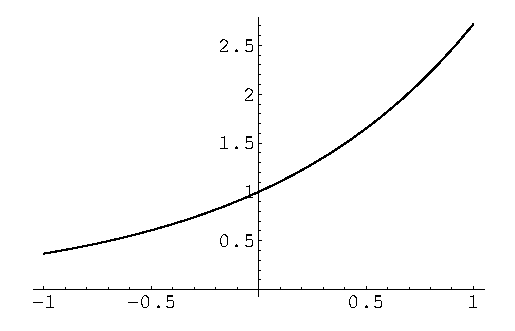
\includegraphics[width=4.0cm]{image4.eps}}
%  \vspace{1.5cm}
  \centerline{(c) Result 4}\medskip
\end{minipage}
%
\caption{Example of placing a figure with experimental results.}
\label{fig:res}
%
\end{figure}


% To start a new column (but not a new page) and help balance the last-page
% column length use \vfill\pagebreak.
% -------------------------------------------------------------------------
%\vfill
%\pagebreak

\vfill\pagebreak




% References should be produced using the bibtex program from suitable
% BiBTeX files (here: strings, refs, manuals). The IEEEbib.bst bibliography
% style file from IEEE produces unsorted bibliography list.
% -------------------------------------------------------------------------
\bibliographystyle{IEEEbib}
\bibliography{strings,refs}

\end{document}
